\documentclass[]{scrartcl}
%\usepackage{graphicx}
%\usepackage{amsmath} % For equation alignment
\usepackage{amssymb} % For special math characters such as E with two vertical lines (expectation value symbol)
\usepackage{mathtools} % For some extra math-related functionality, such as matrix*
%\usepackage{hyperref} % For using \autoref
%\usepackage{listings} % For adding code to the latex document
%\usepackage{caption} % For adding captions
\usepackage{color} % For color in code
\usepackage{nicematrix} % For creating matrices with outer rows and columns, with dsahed line separators. Documentation: https://ctan.org/pkg/nicematrix
%\usepackage{float} % For better control over float environments
%\usepackage[utf8]{inputenc} % this is needed for umlauts
%\usepackage[ngerman]{babel} % this is needed for umlauts
%\usepackage[T1]{fontenc}    % this is needed for correct output of umlauts in pdf




% Opening / Title
\title{Complex Systems for Bioinformaticians \\ \vspace{2mm} Assignment 3 \\ \vspace{2mm}}
\subtitle{Lecturers: Prof. Dr. Max von Kleist, Prof. Dr. Jana Wolf, Prof. Dr. Martin Vingron}
\author{Kristian Reinhart, 4474140 \\ Duong Ha Le Minh, 5314209}
\newenvironment{tightcenter}{%
  \setlength\topsep{0pt}
  \setlength\parskip{0pt}
  \begin{center}
}{%
  \end{center}
}




%%%%%%%%%%%%%%%%%%%%%%%%%%%%%%%%%%%
%%%	Begin actual document	%%%
%%%%%%%%%%%%%%%%%%%%%%%%%%%%%%%%%%%


\begin{document}




\maketitle




\section*{3. Assignment}

%%%%%%%%%%%%%%%
%%%	Task 1	%%%
%%%%%%%%%%%%%%%

\subsection*{Task 1)}

Given the weak law of large numbers the standard deviation of the sample mean $\overline{x}^{(p)}$ can be expressed as
$\sigma_{p} ~ = ~ \sqrt{\mathbb{E} \left[ { \vert \overline{x}^{(n)} ~ - ~ \mu \vert }^{2} \right] }$.
\\
The standard deviation $\sigma_{p}$ shrinks at the order of $\mathcal{O} \left( \dfrac{1}{\sqrt{n}} \right)$, with $n$ being the number of samplings.
\\
\\
This in turn means that in order to double the precision (and thus halving the standard deviation $\sigma_{p}$) the number of sampling $n$ must increase by a factor of 4.
Conversely, to halve the precision (and thus doubling the standard deviation $\sigma_{p}$) the number of sampling $n$ must decrease by a factor of 4.
\\
\\
Therefore for the given sample Poisson process with a sample mean  $\sigma_{p}~=~0.05$ for $p~=~1000$ samplings, halving the precision to a sample mean of  $\sigma_{p}~=~0.1$ would require $p~=~250$ samplings. 
\\
\\
The standard deviation of the sample mean is the square root of its variance:
\[
\sigma_p = \sqrt{\text{Var}(\overline{X}^{(p)})} = \sqrt{\frac{\sigma^2}{p}} = \frac{\sigma}{\sqrt{p}}
\]
For half the precision, the new $\sigma$ should be twice as big,
$\sigma_{p'} = 2 \sigma_p$:
\[
\frac{\sigma}{\sqrt{p'}} = 2 \frac{\sigma}{\sqrt{p}} \implies \frac{1}{\sqrt{p'}} = \frac{2}{\sqrt{p}} \implies \frac{1}{p'} = \frac{4}{p} \implies p' = \frac{p}{4}
\]
So, to double the standard deviation (halve the precision), the number of samples must decrease by a factor of 4. $1000 / 4 = 250$.



%%%%%%%%%%%%%%%%%%%
%%%	Task 2a)	%%%
%%%%%%%%%%%%%%%%%%%

\subsection*{Task 2a)}

Given model and reaction rates $r_0$ and $r_1$ we reconstruct the stoichiometric matrix $S$ and rate function vector $R$.

\begin{center}
\noindent \begin{minipage}{.4\linewidth}
$ Model:~ 
\begin{matrix*}[c]
	r_0 & : & x_0 & \rightarrow & x_1 \\
	r_1 & : & x_1 & \rightarrow & \emptyset
\end{matrix*}
$
\end{minipage}
\noindent \begin{minipage}{.4\linewidth}
$
R =
\begin{pNiceMatrix}[last-col,nullify-dots]
	k_a * x_0 & r_0 \\
	k_e	* x_1 & r_1 \\
\end{pNiceMatrix}
$
\end{minipage}
\end{center}

\noindent
From model and reaction rates we reconstruct the stoichiometric matrix $S$:

% Have the matrix in a float-environment and center it, looks nicer
\noindent \begin{center}
\begin{minipage}{.4\linewidth}
$
S =
\begin{pNiceMatrix}[first-row,last-col,nullify-dots]
	R_0	&	R_1 \\
	 -1 &	  0 &	X_0 \\
	  1 &	 -1 &	X_1 \\
\end{pNiceMatrix}
$
\end{minipage}
\end{center}

\noindent 
Finally, combining the stoichiometric matrix $S$ and rate function vector $R$ we can reconstruct the ODE:

\noindent \begin{center}
\begin{minipage}{.5\linewidth}
$
\begin{matrix*}[c]
	\frac{d}{dt} X_0(t) & = & - & \underbrace{k_a * x_0(t)}	&	& 							\\ 
					    &   &   & 							r_0 &   &							\\
	\frac{d}{dt} X_1(t) & = &   & \underbrace{k_a * x_0(t)}	& - & \underbrace{k_e * x_1(t)}	\\
					    &   &   & 							r_0 &   &					r_1 
\end{matrix*}
$
\end{minipage}
\end{center}



%%%%%%%%%%%%%%%%%%%
%%%	Task 2b)	%%%
%%%%%%%%%%%%%%%%%%%

%\clearpage
\subsection*{Task 2b)}

% Referenzen:
% Page 5+6: https://digitalcommons.augustana.edu/cgi/viewcontent.cgi?article=1001&context=mathstudent
% Page 3+4: https://www.uuappliedandlifesciences.com/wp-content/uploads/2022/12/Paper-9.pdf
% Lecture 6, slide 19?

We begin by solving the ODE for $x_0(t)$.

\begin{align*}
	\frac{d}{dt} x_0(t) &= - k_a * x_0(t) \\
	\frac{1}{x_0(t)} \frac{d}{dt} X_0(t) &= - k_a \\
	\frac{1}{x_0(t)} d X_0(t) &= - k_a dt \\
	\int \frac{1}{x_0(t)} d X_0(t) &= \int - k_a dt \\
	\ln \vert x_0(t) \vert &= - k_a * t + C \\
	x_0(t) &= e^{- k_a * t + C} = e^{- k_a * t} \cdot e^C \\
	x_0(t) &= e^{- k_a * t}
\end{align*}

We will let $A = e^C$

$$
	x_0(t) = Ae^{- k_a * t}
$$

As we know $k_a = 0.5$ and $t_0 = 0$ we can plug in the values and calculate $x_0(t_0)$:

\begin{center}
	$x_0(t_0) ~ = ~ Ae^{- 0.5 * 0} ~ = ~ Ae^0 ~ = ~ A$
\end{center}

As we understand $A$ is equal to our dose, therefore
$$
	x_0(t) = dose \cdot e^{- k_a * t}
$$

Solving for $x_1(t)$:

Substitute $x_0(t)$ into the second ODE:

\begin{align*}
    \frac{dx_1}{dt} &= k_a (\text{dose} \cdot e^{-k_a t}) - k_e x_1\\
    \frac{dx_1}{dt} + k_e x_1 &= k_a \cdot \text{dose} \cdot e^{-k_a t}
\end{align*}

The integrating factor is $I(t) = e^{\int k_e dt} = e^{k_e t}$.
\begin{align*}
e^{k_e t} \frac{dx_1}{dt} + k_e e^{k_e t} x_1 &= k_a \cdot \text{dose} \cdot e^{-k_a t} e^{k_e t}\\
\frac{d}{dt}(x_1 e^{k_e t}) &= k_a \cdot \text{dose} \cdot e^{(k_e - k_a)t}\\
x_1 e^{k_e t} &= \int k_a \cdot \text{dose} \cdot e^{(k_e - k_a)t} dt \\
x_1 e^{k_e t} &= k_a \cdot \text{dose} \cdot \frac{1}{k_e - k_a} e^{(k_e - k_a)t} + C'
\end{align*}

Solve for $x_1(t)$:
\begin{align*}
x_1(t) &= \left( k_a \cdot \text{dose} \cdot \frac{1}{k_e - k_a} e^{(k_e - k_a)t} + C' \right) e^{-k_e t} \\
x_1(t) &= \frac{k_a \cdot \text{dose}}{k_e - k_a} e^{-k_a t} + C' e^{-k_e t}
\end{align*}

$x_1(0) = 0$:

\begin{align*}
0 = \frac{k_a \cdot \text{dose}}{k_e - k_a} e^0 + C' e^0 \implies 0 &= \frac{k_a \cdot \text{dose}}{k_e - k_a} + C'\\
C' = -\frac{k_a \cdot \text{dose}}{k_e - k_a}\\
\end{align*}

\begin{align*}
x_1(t) &= \frac{k_a \cdot \text{dose}}{k_e - k_a} e^{-k_a t} - \frac{k_a \cdot \text{dose}}{k_e - k_a} e^{-k_e t}\\
x_1(t) &= \frac{k_a \cdot \text{dose}}{k_e - k_a} (e^{-k_a t} - e^{-k_e t})\\
\end{align*}
$k_a=0.5$, $k_e=0.3$:
\begin{align*}
x_1(t) &= \frac{0.5 \cdot \text{dose}}{0.3 - 0.5} (e^{-0.5 t} - e^{-0.3 t}) \\
&= \frac{0.5}{-0.2} \cdot \text{dose} \cdot (e^{-0.5 t} - e^{-0.3 t}) \\
&= -2.5 \cdot \text{dose} \cdot (e^{-0.5 t} - e^{-0.3 t}) \\
x_1(t) &= 2.5 \cdot \text{dose} \cdot (e^{-0.3 t} - e^{-0.5 t})
\end{align*}

%%%%%%%%%%%%%%%%%%%
%%%	Task 3b)	%%%
%%%%%%%%%%%%%%%%%%%

\clearpage
\subsection*{Task 3b)}

\begin{figure}[htbp!]
	\centering
	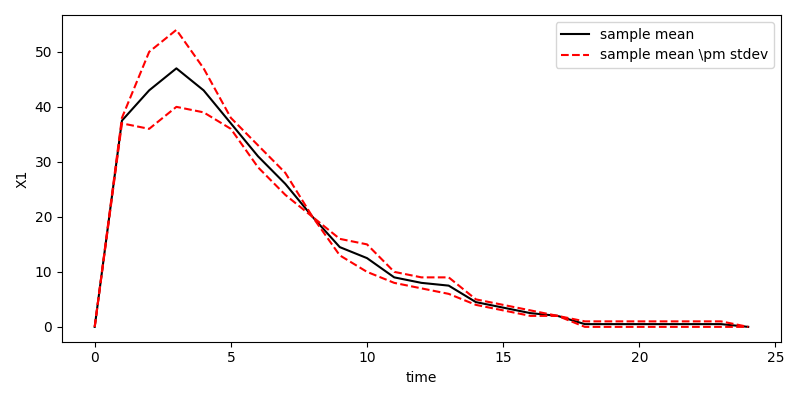
\includegraphics[width=0.6\textwidth]{Exercise3Homework3b.png}
	\caption{100 simulations of the pharmacokinetic model of homework 2.
			 The black line indicates the sample mean $\overline{x}(t)$ and the red dotted lines mark the sample mean $\pm$ one standard deviation.}
\end{figure}



%%%%%%%%%%%%%%%%%%%
%%%	Task 3d)	%%%
%%%%%%%%%%%%%%%%%%%
\clearpage
\subsection*{Task 3d)}

\textbf{\textcolor{red}{TODO: Add plot and discuss order at which error $\epsilon$ tends to zero as a function of $N$, e.g. $\mathcal{O}(?)$}}

\begin{figure}[htbp!]
	\centering
	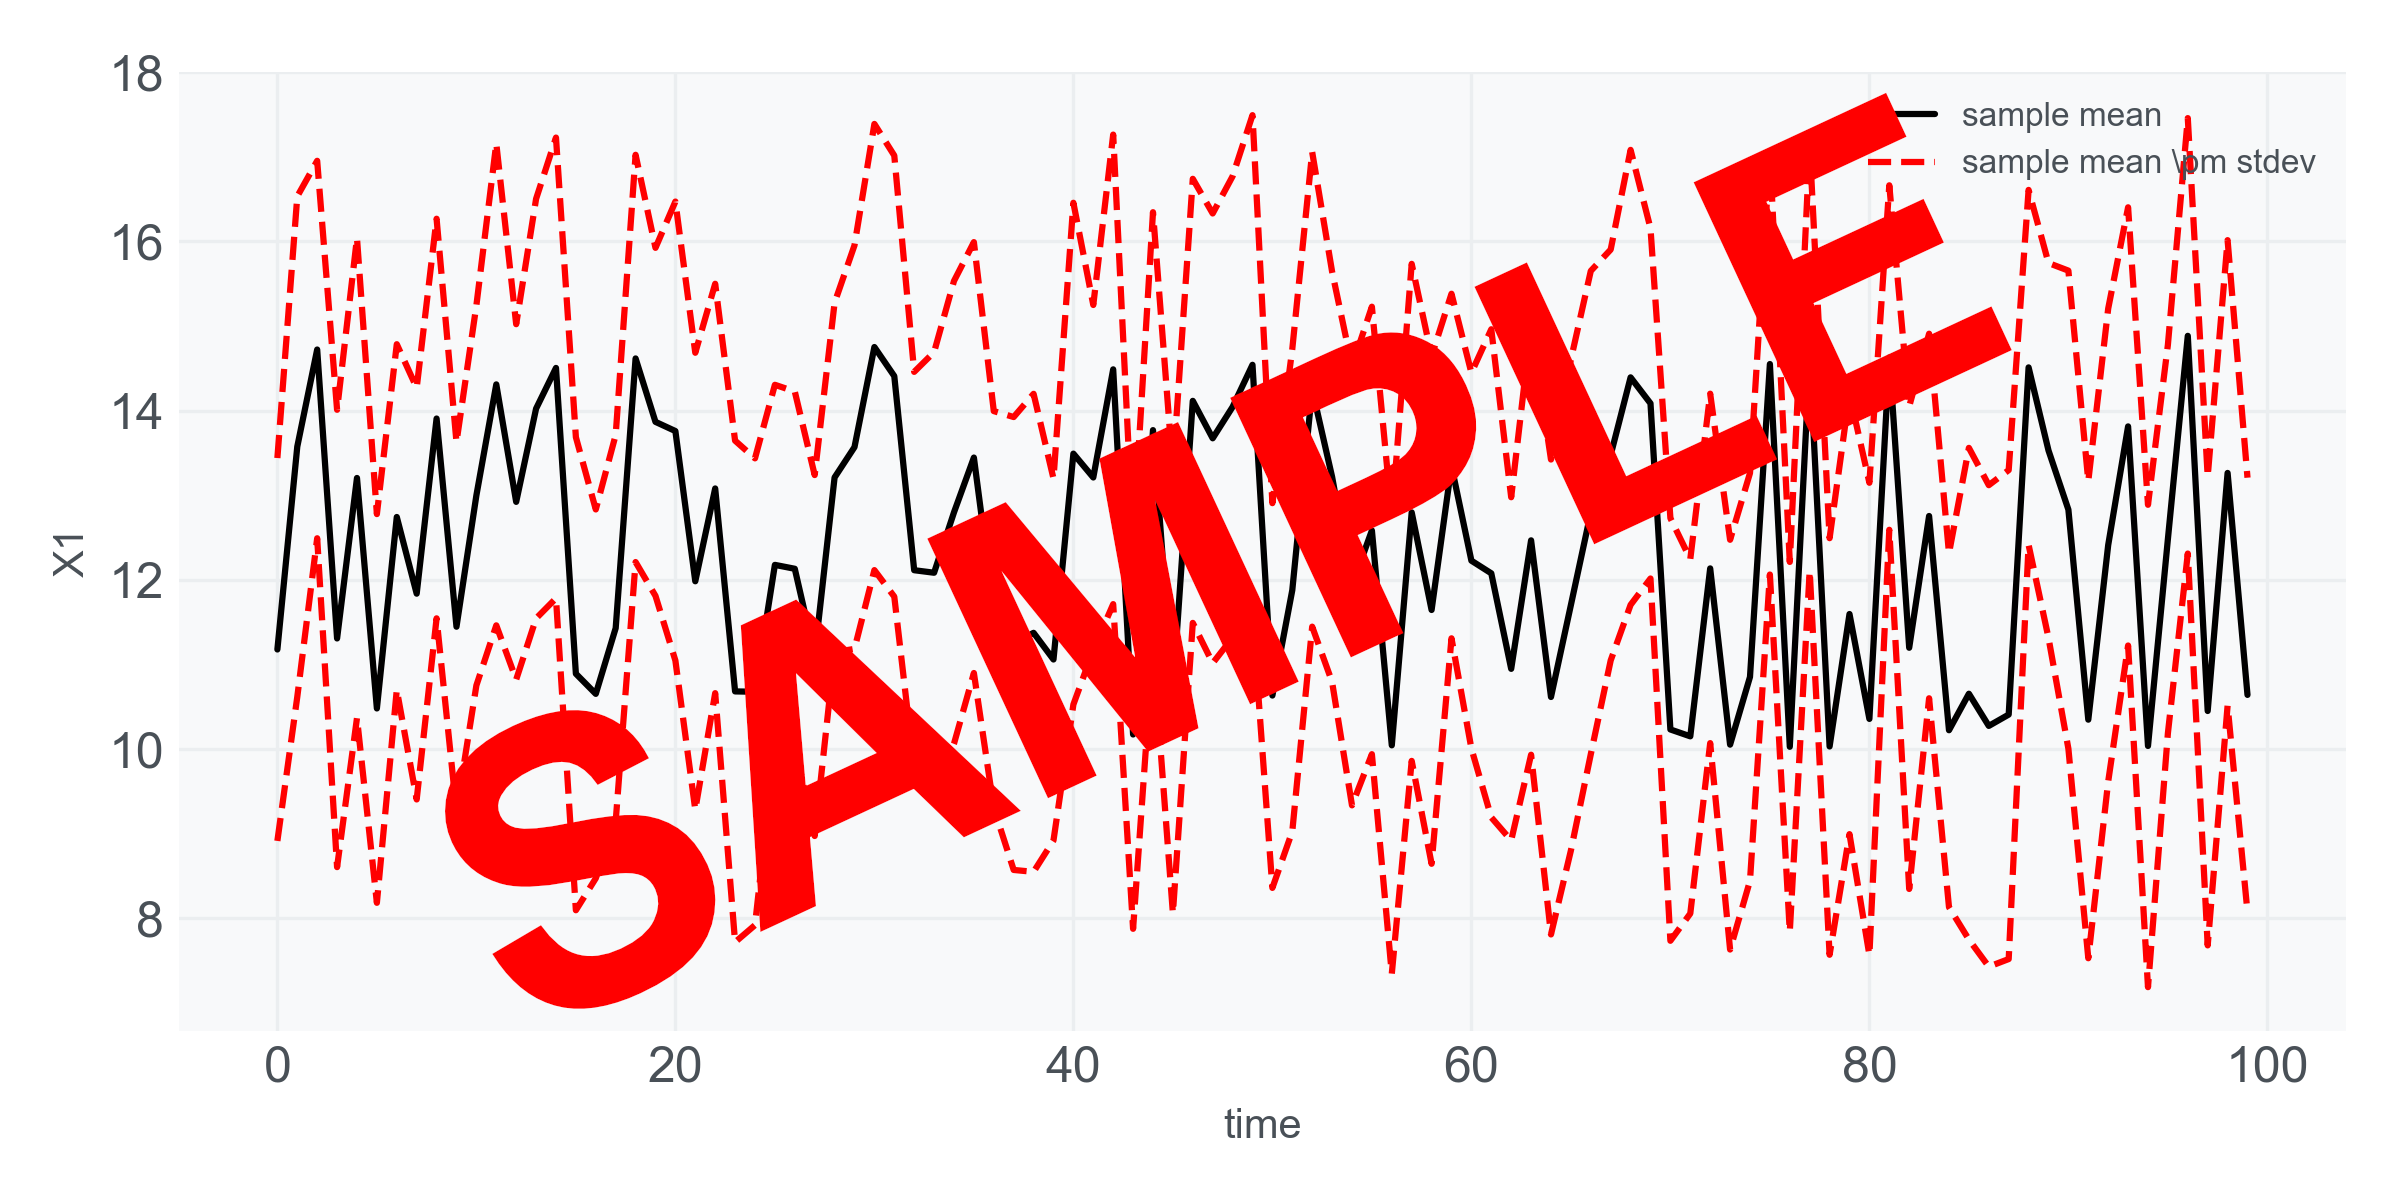
\includegraphics[width=0.6\textwidth]{Exercise3Homework3d.png}
	\caption{ \textbf{\textcolor{red}{TODO: Add caption for plot. Don't know how it'll look, so placeholder.}} }
\end{figure}


\end{document}

